\documentclass[tikz,border=12pt]{standalone}
\usepackage{tikz}
\usetikzlibrary{shapes.geometric,arrows.meta,positioning,fit,backgrounds,calc}

\renewcommand{\familydefault}{\sfdefault}
\definecolor{cborder}{HTML}{1E293B}
\definecolor{cbg}{HTML}{F8FAFC}
\definecolor{cbox}{HTML}{FFFFFF}
\definecolor{cblue}{HTML}{1E40AF}
\definecolor{cbluelight}{HTML}{EFF6FF}
\definecolor{cgray}{HTML}{64748B}
\definecolor{camberbg}{HTML}{F1F5F9}

\begin{document}
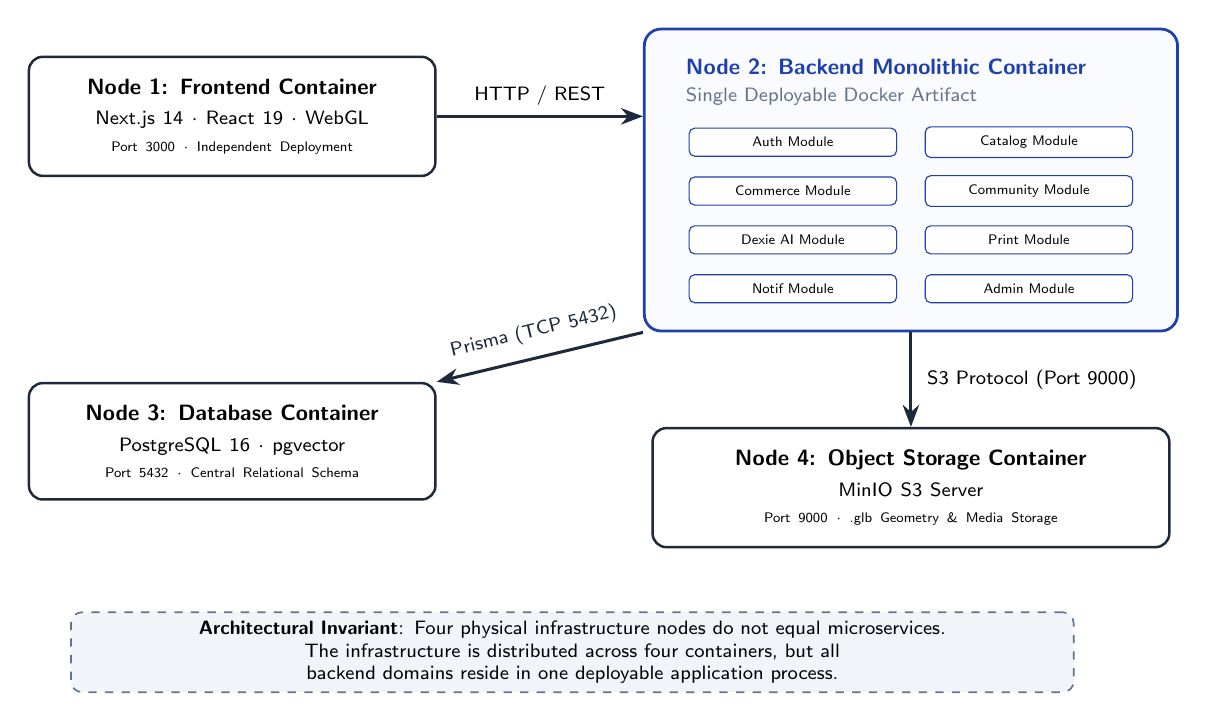
\begin{tikzpicture}[
    font=\small,
    >=Stealth,
    node distance=1.2cm and 2.0cm,
    nodebox/.style={
        draw=cborder,
        fill=white,
        rounded corners=5pt,
        line width=0.9pt,
        align=center,
        inner sep=8pt,
        font=\footnotesize
    },
    flow/.style={
        ->,
        line width=1.1pt,
        draw=cborder
    }
]

    % Node 1: Frontend (Top Left)
    \node[nodebox, text width=4.6cm] (n1) {
        \textbf{Node 1: Frontend Container}\\[3pt]
        \scriptsize Next.js 14 $\cdot$ React 19 $\cdot$ WebGL\\
        \tiny Port 3000 $\cdot$ Independent Deployment
    };

    % Node 3: Database (Bottom Left)
    \node[nodebox, below=2.6cm of n1, text width=4.6cm] (n3) {
        \textbf{Node 3: Database Container}\\[3pt]
        \scriptsize PostgreSQL 16 $\cdot$ pgvector\\
        \tiny Port 5432 $\cdot$ Central Relational Schema
    };

    % Node 2 Modules (Top Right)
    \node[draw=cblue, fill=white, rounded corners=2pt, font=\tiny, text width=2.4cm, align=center, right=3.2cm of n1.north east, yshift=-1.1cm] (m1) {Auth Module};
    \node[draw=cblue, fill=white, rounded corners=2pt, font=\tiny, text width=2.4cm, align=center, right=0.35cm of m1] (m2) {Catalog Module};
    \node[draw=cblue, fill=white, rounded corners=2pt, font=\tiny, text width=2.4cm, align=center, below=0.25cm of m1] (m3) {Commerce Module};
    \node[draw=cblue, fill=white, rounded corners=2pt, font=\tiny, text width=2.4cm, align=center, right=0.35cm of m3] (m4) {Community Module};
    \node[draw=cblue, fill=white, rounded corners=2pt, font=\tiny, text width=2.4cm, align=center, below=0.25cm of m3] (m5) {Dexie AI Module};
    \node[draw=cblue, fill=white, rounded corners=2pt, font=\tiny, text width=2.4cm, align=center, right=0.35cm of m5] (m6) {Print Module};
    \node[draw=cblue, fill=white, rounded corners=2pt, font=\tiny, text width=2.4cm, align=center, below=0.25cm of m5] (m7) {Notif Module};
    \node[draw=cblue, fill=white, rounded corners=2pt, font=\tiny, text width=2.4cm, align=center, right=0.35cm of m7] (m8) {Admin Module};

    % Header spacer coordinate to give title plenty of room
    \coordinate[above=0.9cm of m1.north west] (n2_top_pad);

    % Node 2 Container (Top Right)
    \begin{scope}[on background layer]
        \node[draw=cblue, fill=cbluelight!40, rounded corners=6pt, line width=1pt,
              fit=(n2_top_pad) (m1) (m2) (m3) (m4) (m5) (m6) (m7) (m8),
              inner xsep=16pt, inner ysep=10pt] (n2) {};
    \end{scope}

    \node[anchor=north west, font=\bfseries\footnotesize, text=cblue, align=left] at (n2.north west) [xshift=12pt, yshift=-8pt] {
        Node 2: Backend Monolithic Container\\
        \scriptsize\mdseries\color{cgray} Single Deployable Docker Artifact
    };

    % Node 4: Object Storage (Bottom Right)
    \node[nodebox, below=1.2cm of n2, text width=6.0cm] (n4) {
        \textbf{Node 4: Object Storage Container}\\[3pt]
        \scriptsize MinIO S3 Server\\
        \tiny Port 9000 $\cdot$ .glb Geometry \& Media Storage
    };

    % Connections
    \draw[flow] (n1) -- (n1 -| n2.west) node[midway, above, font=\scriptsize] {HTTP / REST};
    
    % Clean direct route to Node 3
    \draw[flow] (n2.south west) -- node[midway, sloped, above=2pt, font=\scriptsize, text=cborder] {Prisma (TCP 5432)} (n3.north east);

    % Clean route to Node 4
    \draw[flow] (n2.south -| n4.north) -- (n4.north)
        node[midway, right, font=\scriptsize, xshift=2pt] {S3 Protocol (Port 9000)};

    % Architectural Invariant Note at Bottom
    \node[draw=cgray, fill=camberbg, rounded corners=4pt, dashed, line width=0.6pt,
          below=0.8cm of n4, text width=12.5cm, align=center, font=\scriptsize, xshift=-4.3cm] (note) {
        \textbf{Architectural Invariant}: Four physical infrastructure nodes do not equal microservices.\\
        The infrastructure is distributed across four containers, but all backend domains reside in one deployable application process.
    };

\end{tikzpicture}
\end{document}
